\documentclass{article}                                                         
\usepackage[french]{babel}
\usepackage[final]{pdfpages}
\usepackage{geometry}
\geometry{hmargin=2.5cm,vmargin=1.5cm}
\usepackage[T1]{fontenc}                                                        
\usepackage[utf8x]{inputenc}                                                    
\usepackage{algorithmeUTF8}                                                     
\title{RAPPORT PROJET OTHELLO}                         
\author{Victorin Turnel, Paul Thulliez,Chen Yang, Ahmed Zarki, Sacha Wojciechowski}

\begin{document}
\maketitle



\section{Analyse}

\subsection{TAD COULEUR :}
\begin{tad}
\tadNom{Couleur}
\tadDependances{Booleen}

\begin{tadOperations}{couleur}  
\tadOperation{blanc}{\tadUnParam{Couleur}}
\tadOperation{noir}{\tadUnParam{Couleur}}
\tadOperation{estBlanc}{\tadUnParam{Couleur}}{\tadUnParam{Booleen}}
\tadOperation{changerCouleur}{\tadUnParam{Couleur}}{\tadUnParam{Couleur}}
\end{tadOperations}

\begin{tadAxiomes}
\tadAxiome{estBlanc(blanc())}
\tadAxiome{non(estBlanc(noir()))}
\tadAxiome{changerCouleur(blanc())=noir()}
\end{tadAxiomes}

\end{tad}

\subsection{TAD PION :}
\begin{tad}
\tadNom{Pion}
\tadDependances{Couleur}

\begin{tadOperations}{creerPion}  
\tadOperation{creerPion}{\tadUnParam{Couleur}}{\tadUnParam{Pion}}
\tadOperation{obtenirCouleurSuperieure}{\tadUnParam{Pion}}{\tadUnParam{Couleur}}
\tadOperation{retournerPion}{\tadUnParam{Pion}}{\tadUnParam{Pion}}
\end{tadOperations}

\begin{tadAxiomes}
\tadAxiome{obtenirCouleurSuperieure(retournerPion(creerPion(col) != col}
\end{tadAxiomes}

\end{tad}


\subsection{TAD POSITION :}
\begin{tad}
	\tadNom{Position}
	\tadDependances{1..8}
	\begin{tadOperations}{Position}
		\tadOperation{position}{\tadDeuxParams{1..8}{1..8}}{Position}
		\tadOperation{obtenirX}{Position}{1..8}
		\tadOperation{obtenirY}{Position}{1..8}
	\end{tadOperations}
	\begin{tadAxiomes}
		\tadAxiome{obtenirX(Position(x,y))=x}
		\tadAxiome{obtenirY(Position(x,y))=y}
	\end{tadAxiomes}
	
	
\end{tad}


\subsection{TAD COUP :}
\begin{tad}
	\tadNom{Coup}
	\tadDependances{Pion,Pion,Position}
	\begin{tadOperations}{Coup}
		\tadOperation{coup}{Pion,Position}{\tadUnParam{Coup}}
		\tadOperationAvecPreconditions{obtenirPionCoup}{Coup}{Pion}
		\tadOperationAvecPreconditions{obtenirPositionCoup}{\tadUnParam{Coup}}{Position}
        \end{tadOperations}
              
	\begin{tadAxiomes}
          \tadAxiome{obtenirPionCoup(coup(pion,pos))=pion}
          \tadAxiome{obtenirPositionCoup(coup(pion,pos))=pos}
	\end{tadAxiomes}


\end{tad}

\subsection{TAD COUPS :}
\begin{tad}
	\tadNom{Coups}
	\tadDependances{Coup, NNN, Naturel}
	\begin{tadOperations}{Coups}
		\tadOperation{coups}{}{\tadUnParam{Coups}}
		\tadOperation{nbCoups}{Coups}{Naturel}
		\tadOperation{ajouterCoups}{\tadDeuxParams{Coups}{Coup}}{Coups}
		\tadOperationAvecPreconditions{iemeCoup}{\tadDeuxParams{Coups}{NNN}}{Coup}
	\end{tadOperations}
	\begin{tadPreconditions}{Coups}
		\tadPrecondition{iemeCoups(coups,position)}{position $\leq$ nbCoups(coups)}
	\end{tadPreconditions}
	\begin{tadAxiomes}
		\tadAxiome{nbCoups(Coups())=0}
		\tadAxiome{nbCoups(ajouterCoups(coups,coup)) = nbCoups(coups) +1}
		\tadAxiome{iemeCoup(ajouterCoups(coups,coup),nbCoups(coups)+1 ) = coup}
	\end{tadAxiomes}


\end{tad}
        


\subsection{TAD PLATEAU :}

\begin{tad}


\tadNom{Plateau}
\tadDependances{Pion, Position, \booleen}

\begin{tadOperations}{retournerPion}
	\tadOperation{plateau}{}{\tadUnParam{Plateau}}
	\tadOperationAvecPreconditions{poserPion}{\tadTroisParams{Plateau}{Position}{Pion}}{\tadUnParam{Plateau}}
	\tadOperationAvecPreconditions{obtenirPion}{\tadDeuxParams{Plateau}{Position}}{\tadUnParam{Pion}}
	\tadOperation{estCaseVide}{\tadDeuxParams{Plateau}{Position}}{\tadUnParam{\booleen}}
	\tadOperationAvecPreconditions{retournerPion}{\tadDeuxParams{Plateau}{Position}}{\tadUnParam{Plateau}}
	\tadOperationAvecPreconditions{enleverPion}{\tadDeuxParams{Plateau}{Position}}{\tadUnParam{Plateau}}
\end{tadOperations}

\begin{tadPreconditions}{poserPion(pos,pion,pl)}
	\tadPrecondition{obtenirPion(pos,pl)}{non (estCaseVide(pos,pl))}	
	\tadPrecondition{retournerPion(pos,pl)}{non (estCaseVide(pos,pl))}
	\tadPrecondition{poserPion(pos,pion,pl)}{estCaseVide(pos,pl)}
	\tadPrecondition{enleverPion(pos,pl)}{non (estCaseVide(pos,pl))}
\end{tadPreconditions}

\begin{tadAxiomes}
	\tadAxiome{estCaseVide(pos,plateau())}
	\tadAxiome{obtenirPion(pos,poserPion(pos,pion,plateau()))= pion}
	\tadAxiome{estCaseVide(pos,enleverPion(pos,plateau()))}
	\tadAxiome{non estCaseVide(pos,poserPion(pos,pion,plateau()))}
	\tadAxiome{retournerPion(pos,retournerPion(pos,pl))=pl}	
\end{tadAxiomes}
\end{tad}


\subsection{Analyse descendante de la fonction faireUnePartie}
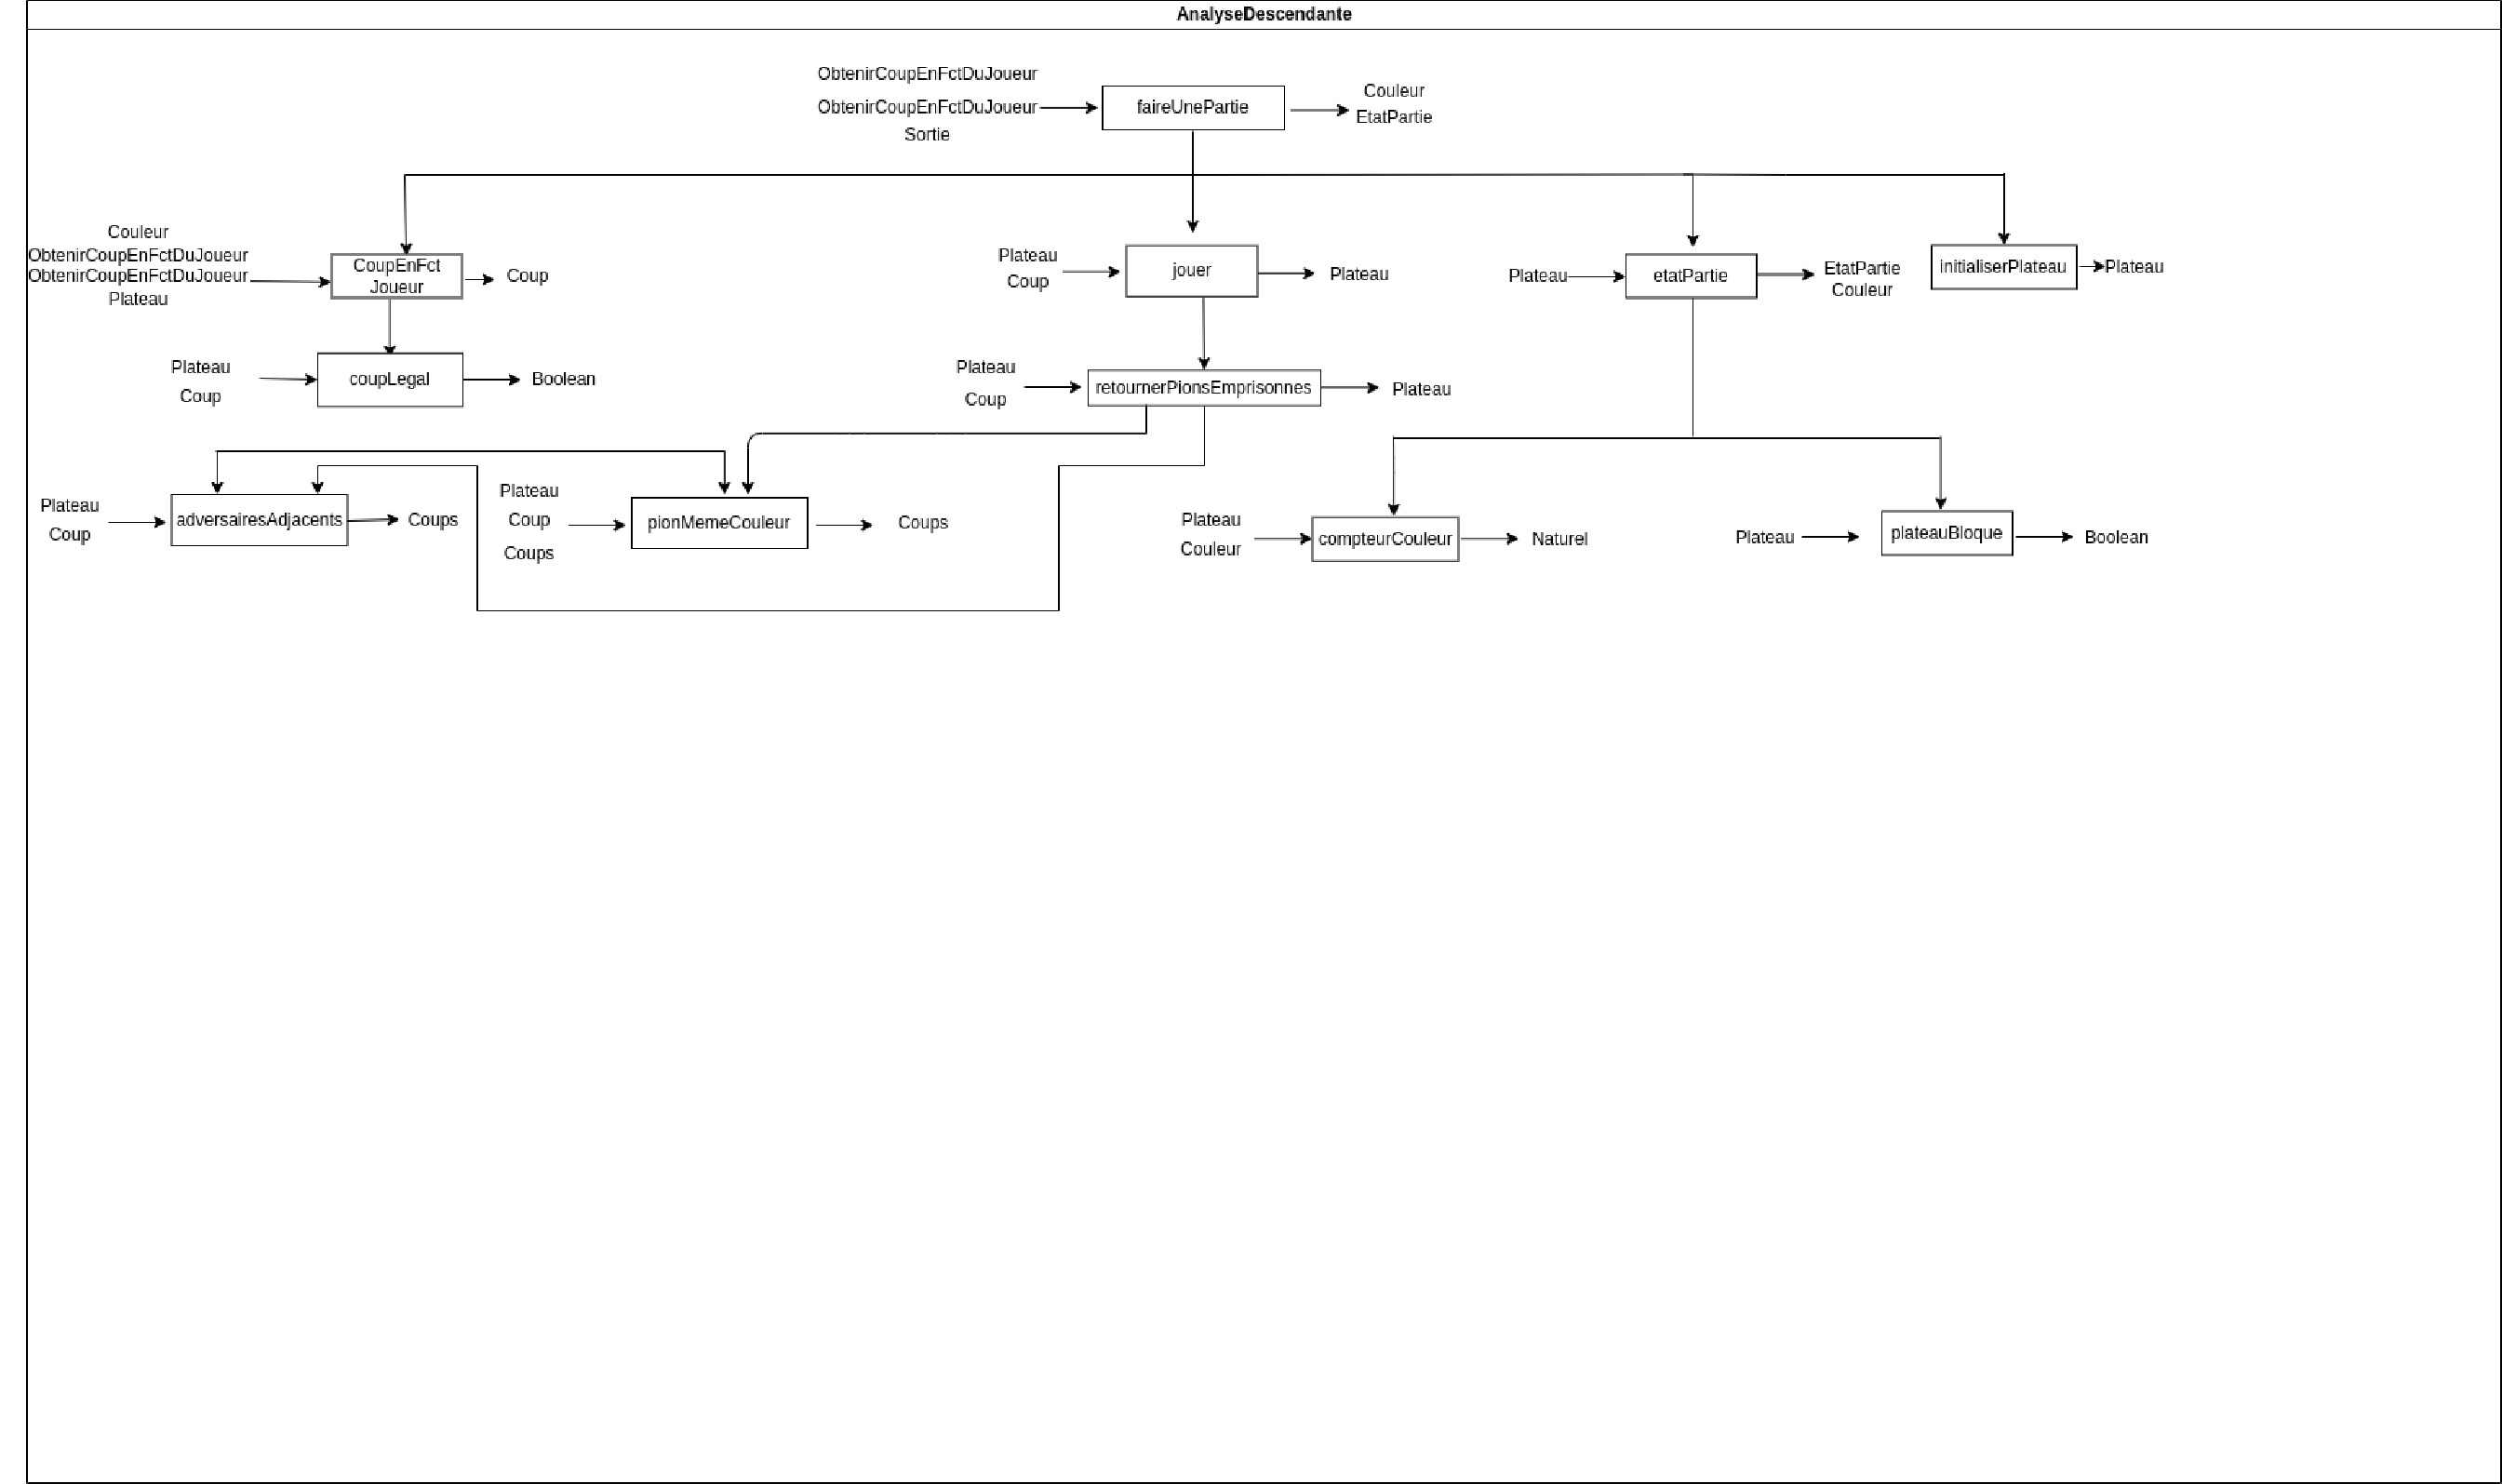
\includepdf{analyse/ADfaireUnePartie.pdf}

\subsection{Analyse descendante de la fonction obtenirCoup}



\section{Conception préliminaire}

\subsection{TAD : Couleur}
\begin{algorithme}
	\signaturefonction{couleurBlanc}{}{Couleur}
	\signaturefonction{couleurNoir}{}{Couleur}
	\signaturefonction{couleurEstBlanc}{c : Couleur}{\booleen}
  	\signaturefonction{couleurChangerCouleur}{couleur:Couleur}{Couleur}
\end{algorithme}


\subsection{TAD : Pion}
\begin{algorithme}
  \signaturefonction{creerPion}{couleur : Couleur}{Pion}
  \signaturefonction{obtenirCouleurSuperieure}{pion : Pion}{Couleur}
  \signatureprocedure{retournerPion}{\paramEntree{pion : Pion},\paramSortie{Pion}}
\end{algorithme}
  


\subsection{TAD : Position}
\begin{algorithme}
	\signaturefonction
	{position}
	{largeur : \textbf{1..8}, hauteur : \textbf{1..8}}
	{\textbf{Position}}
	
	\vspace*{5mm}
	
	\signaturefonction
	{obtenirX}
	{unePosition : \textbf{Position}}
	{\textbf{1..8}}
	
	\vspace*{5mm}
	
	\signaturefonction
	{obtenirY}
	{unePosition : \textbf{Position}}
	{\textbf{1..8}}
	
	
	
\end{algorithme}




\subsection{TAD : Coup}
\begin{algorithme}
\signaturefonction{coupCoup}{pion:Pion}{Coup}
\signaturefonction{coupObtenirPionCoup}{coup:Coup}{Pion}
\signaturefonction{coupObtenirPositionCoup}{coup:Coup}{Position}
\end{algorithme}


\subsection{TAD : Coups}
\begin{algorithme}
	\signaturefonction
	{coups}
	{}
	{\textbf{Coups}}
	
	\vspace*{5mm}
	
	\signaturefonction
	{nbCoups}
	{cps : \textbf{Coups}}
	{\naturel}
	
	\vspace*{5mm}
	
	\signatureprocedure
	{ajouterCoups}
	{\paramEntreeSortie{cps : \textbf{Coups}},\paramEntree{unCoup : \textbf{Coup}}}
	
	\vspace*{5mm}
	
	\signaturefonction
	{iemeCoup}
	{cps : \textbf{Coups}, place : \textbf{NNN}}
	{\textbf{Coup}}
	\preconditions{place $\leq$ nbCoups(coups)}
	
	
	
\end{algorithme}


\subsection{TAD : Plateau}
\begin{algorithme}
  \signaturefonction{plateau}{}{Plateau}
  \signatureprocedure{poserPion}{\paramEntreeSortie{plateau : Plateau} , \paramEntree{pos : Position , pion: Pion}}

  \vspace*{5mm}
  
  \preconditions{estCaseVide(plateau , pos)}

  \vspace*{5mm}
  
  \signaturefonction{obtenirPion}{plateau : Plateau , pos : Position}{Pion}

  \vspace*{5mm}

  \preconditions{non (estCaseVide(plateau , pos)}

  \vspace*{5mm}
  
  \signaturefonction{estCaseVide}{plateau : Plateau , pos : Position}{\booleen}

  \vspace*{5mm}
  
  \signatureprocedure{retournerPion}{\paramEntreeSortie{plateau : Plateau} , \paramEntree{pos : Position}}

  \vspace*{5mm}
  
  \preconditions{non (estCaseVide(plateau , pos)}

  \vspace*{5mm}
  
  \signatureprocedure{enleverPion}{\paramEntreeSortie{plateau : Plateau},\paramEntree{pos : Position}}

  \vspace*{5mm}
  
  \preconditions{non (estCaseVide(plateau , pos)}
\end{algorithme}


\subsection{faireUnePartie}
\begin{algorithme}
  \type{EtatPartie}{[TERMINE,ENCOURS,EGALITE]}
\end{algorithme}

\vspace*{5mm}

\begin{algorithme}
  \type{Sortie}{\signatureprocedure{}{\paramEntree{plateau : \textbf{Plateau}, coup : \textbf{Coup}, possibilite : \booleen}}}
\end{algorithme}

\vspace*{5mm}

\begin{algorithme}
  \type{ObtenirCoupEnFctDuJoueur}{\signaturefonction{}{plateau : \textbf{Plateau}, joueur : \textbf{Couleur}, profondeur:\naturel}}{\textbf{Coup}}
\end{algorithme}

\vspace*{5mm}

\begin{algorithme}
  \signatureprocedure{faireUnePartie}{\paramEntree{obtenirCoupBlanc,obtenirCoupJoueurNoir : \textbf{ObtenirCoupEnFctDuJoueur}, sortie : \textbf{Sortie}} \paramSortie{couleurGagnant : \textbf{Couleur}, etat : \textbf{EtatPartie}}}
  
  \vspace*{5mm}
  
  \signaturefonction{initialiserPlateau}{}{\textbf{Plateau}}

  \vspace*{5mm}
  
  \signatureprocedure{etatPartie}{\paramEntree{plateau : \textbf{Plateau}}, \paramSortie{couleur: \textbf{Couleur}, etat: \textbf{EtatPartie}}}

  \vspace*{5mm}
  
  \signaturefonction{compteurCouleur}{plateau : \textbf{Plateau}, couleur : \textbf{Couleur}}{\naturel}

  \vspace*{5mm}
  
  \signaturefonction{plateauBloque}{plateau : \textbf{Plateau}}{\booleen}

  \vspace*{5mm}
  
  \signatureprocedure{jouer}{\paramEntreeSortie {plateau : \textbf{Plateau}} , \paramEntree{coup : \textbf{Coup}}}
  
  \vspace*{5mm}
  
  \signaturefonction{coupLegal}{plateau : \textbf{Plateau} , coup : \textbf{Coup}}{\booleen}

  \vspace*{5mm}
  \signatureprocedure{retournerPionsEmprisonnes}{\paramEntreeSortie{plateau : \textbf{Plateau}} , \paramEntree{coup : \textbf{Coup}}}

  \vspace*{5mm}
  
  \signaturefonction{adversairesAdjacents}{plateau : \textbf{Plateau} , coup : \textbf{Coup}}{\textbf{Coups}}

  \vspace*{5mm}
  
  \signaturefonction{pionMemeCouleur}{plateau : \textbf{Plateau} , coup : \textbf{Coup}, pionsLegals : \textbf{Coups}}{\textbf{Coups}}

  \vspace*{5mm}
  
  \signaturefonction{coupEnFctJoueur}{obtenirCoupBlanc,obtenirCoupNoir : \textbf{ObtenirCoupEnFctDuJoueur}, couleur : \textbf{Couleur}, plateau : \textbf{Plateau}}{\textbf{Coup}}
\end{algorithme}



\subsection{obtenirCoup}
\begin{algorithme}
	\signaturefonction
	{obtenirCoups}
	{unPlateau : \textbf{Plateau}, joueur : \textbf{Pion}, profondeur : \naturel}
	{\textbf{Coup}}
	\preconditions{non plateauComplet(unPlateau)}

	\vspace*{5mm}

	\signaturefonction
	{scoreDUnCoup}
	{unPlateau : \textbf{Plateau}, joueurRef, joueurCourant : \textbf{Pion}, unCoup : \textbf{Coup},profondeur : \naturel}
	{\entier}
	
	\vspace*{5mm}
	
	\signaturefonction
	{alphaBeta}
	{unPlateau : \textbf{Plateau}, joueurRef, joueurCourant : \textbf{Pion}, profondeur : \naturel, alpha, beta : \entier}
	{\entier}
	
	\vspace*{5mm}
	
	\signaturefonction
	{plateauComplet}
	{unPlateau : \textbf{Plateau}}
	{\booleen}
	
	\vspace*{5mm}
	
	\signaturefonction
	{coupGagnant}
	{unPlateau : \textbf{Plateau}, unCoup : \textbf{Coup}}
	{\booleen}
	
	\vspace*{5mm}
	
	\signaturefonction
	{évaluer}
	{unPlateau : \textbf{Plateau}, joueurRef : \textbf{Pion}}
	{\entier}
	
	\vspace*{5mm}
	
	\signaturefonction
	{score}
	{unPlateau : \textbf{Plateau}, joueur : \textbf{Pion}}
	{\entier}
	
	\vspace*{5mm}
	
	\signaturefonction
	{obtenirCoupsPossibles}
	{unPlateau : \textbf{Plateau}}
	{\textbf{Coups}}
	

	
\end{algorithme}

	





\section{Conception détaillé}
\subsection{TAD : Couleur}
\begin{algorithme}
  \type{Couleur}{\{Blanc,Noir\}}
\end{algorithme}

  \vspace*{5mm}


\begin{algorithme}
  \small
  \fonction{blanc}{}{Couleur}
  {}
    {\retourner{Blanc}}

\end{algorithme}


  \vspace*{5mm}

\begin{algorithme}
  \small
  \fonction{noir}{}{Couleur}
  {}
   {\retourner{Noir}}

\end{algorithme}

  \vspace*{5mm}

\begin{algorithme}
  \small
  \fonction{estBlanc}{couleur:Couleur}{\booleen}
  {}
  {\retourner{couleur=Blanc}}

\end{algorithme}

  \vspace*{5mm}

\begin{algorithme}
  \small
  \fonction{changerCouleur}{couleur:Couleur}{Couleur}
  {}
  {\sialorssinon{estBlanc(couleur)}{\affecter{couleur}{Noir} \retourner{couleur}}{\affecter{couleur}{Blanc} \retourner{couleur}}}

\end{algorithme}


\subsection{TAD : Pion}
\begin{algorithme}
  \begin{enregistrement}{\textbf{Pion}}
    \champEnregistrement{couleur : \textbf{Couleur}}
  \end{enregistrement}
\end{algorithme}

\vspace*{5mm} 

\begin{algorithme}
  \small
  \fonction
      {creerPion}
      {couleur : \textbf{Couleur}}
      {\textbf{Pion}}
      {pion : \textbf{Pion}}
      {{\affecter{pion.Couleur}{couleur}}

        {\retourner {pion}}}
\end{algorithme}

\vspace*{5mm} 

\begin{algorithme}
  \small
  \fonction
      {obtenirCouleurSuperieure}
      {pion : \textbf{Pion}}
      {\textbf{Couleur}}
      {couleur : \textbf{Couleur}}
      {\retourner {pion.Couleur}}
\end{algorithme}

\vspace*{5mm} 

\begin{algorithme}
  \small
  \procedure
      {retournerPion}
      {\paramEntreeSortie{pion : \textbf{Pion}}}
      {}
      {\instruction{changeCouleur(pion.Couleur)}}
\end{algorithme}


\subsection{TAD : Position}
\begin{algorithme}
	
	\begin{enregistrement}{Pion}
		\champEnregistrement{x}{\textbf{1..LARGEUR\_PLATEAU}}
		\champEnregistrement{y}{\textbf{1..HAUTEUR\_PLATEAU}}
	\end{enregistrement}
	
	\vspace*{5mm} 
	
	\fonction
	{position}
	{largeur : \textbf{1..LARGEUR\_PLATEAU}, hauteur : \textbf{1..HAUTEUR\_PLATEAU}}
	{\textbf{Position}}
	{resultat : Position}
	{\affecter{resultat.x}{largeur}
		\affecter{resultat.y}{hauteur}
		\retourner {resultat}}
	
	\vspace*{5mm} 
	
	\fonction
	{obtenirX}
	{unePosition : \textbf{Position}}
	{\textbf{1..LARGEUR\_PLATEAU}}
	{}
	{\retourner {pion.x}}
	
	\vspace*{5mm} 
	
	\fonction
	{obtenirY}
	{unePosition : \textbf{Position}}
	{\textbf{1..HAUTEUR\_PLATEAU}}
	{}
	{\retourner {pion.y}}
	
	
\end{algorithme}

\subsection{TAD : Coup}
\begin{algorithme}
  \begin{enregistrement}{\textbf{Coup}}
    \champEnregistrement{pion}{\textbf{Pion}}
    \champEnregistrement{position}{\textbf{Position}}
  \end{enregistrement}
\end{algorithme}

\vspace*{5mm}

\begin{algorithme}
  \small
  \fonction
      {coupCoup}
      {pion :\textbf{Pion}, pos : \textbf{Position}}
      {\textbf{Coup}}
      {}
      {
        \affecter{coup.position}{pos}
        \affecter{coup.pion}{pion}
        \retourner{coup}
      }
      
\end{algorithme}

\vspace*{5mm}

\begin{algorithme}
  \small
  \fonction
      {coupObtenirPionCoup}
      {coup : \textbf{Coup}}
      {\textbf{Pion}}
      {}
      {
        \retourner{coup.pion} 
      }
      
\end{algorithme}

\vspace*{5mm}

\begin{algorithme}
  \small
  \fonction
      {coupObtenirPositionCoup}
      {coup : \textbf{Coup}}
      {\textbf{Position}}
      {}
      {
        \retourner{coup.position}
      }
      
\end{algorithme}
   

\subsection{TAD : Coups}                                                                              
\begin{algorithme}
	
	\begin{enregistrement}{Coups}
		\champEnregistrement{lesCoups}{\textbf{Tableau[1..LARGEUR\_PLATEAU*HAUTEUR\_PLATEAU] de Coup}}
		\champEnregistrement{nbTotalCoups}{\naturel}
	\end{enregistrement}
	
	\vspace*{5mm} 
	
	\fonction
	{coups}
	{}
	{\textbf{Coups}}
	{resultat : Coups}
	{\affecter{resultat.nbTotalCoups}{0}
		\retourner {resultat}}
	
	\vspace*{5mm} 
	
	\fonction
	{nbCoups}
	{cps : \textbf{Coups}}
	{\naturel}
	{}
	{\retourner {cps.nbTotalCoups}}
	
	\vspace*{5mm} 
	
	\procedure
	{ajouterCoups}
	{\paramEntreeSortie{cps : \textbf{Coups}},\paramEntree{unCoup : \textbf{Coup}}}
	{}
	{\affecter{cps.nbTotalCoups}{cps.nbTotalCoups+1}
		\affecter{cps.lesCoups[cps.nbTotalCoups]}{unCoup}}
	
	\vspace*{5mm} 
	
	\fonction
	{iemeCoup}
	{cps : \textbf{Coups}, place : \textbf{NNN} }
	{\textbf{Coup}
		\preconditions{place $\leq$ nbCoups(coups)}}
	{}
	{\retourner {cps.lesCoups[place]}}
	
	
\end{algorithme}                                                                      





\section{Repartition des tâches}
\begin{tabular}{|l|c|c|c|c|c|}
  \hline
  Tâches & Ahmed Zarki & Victorin Turnel & Chen Yang & Paul Thulliez & Sacha Wojciechowski \\
  \hline
  TAD Couleur  & & & X & X &   \\
  TAD Pion & & & & & X \\
  TAD Position & & X & & &   \\ 
  TAD Coup & & & & X & \\
  TAD Coups & & X  & & &  \\
  TAD Plateau & X & & & & \\
  CP TAD Couleur & & & X & X & \\
  CP TAD Pion & & & & & X \\
  CP TAD Postion & & X & & &  \\
  CP TAD Coup & & & & X & \\
  CP TAD Coups & & X & & & \\
  CP TAD Plateau & X & & & & \\
  Mise en page rapport & & & & & X \\
  Création Makefile & & & & & X \\
  \hline
\end{tabular}



\end{document}
